\par
\bigskip
El filtro miniatura busca crear un efecto de miniaturizacion de una seccion de una imagen. Esto se logra mediante la aplicacion de un filtro de blureado de pixeles a una banda superior e inferior de la imagen, creando de esta forma en la banda central un efecto de miniatura. 

El filtro de blureado se basa en la aplicacion de una matriz de coeficientes a los pixeles circundantes al pixel objetivo y el cambio de los valores de color del mismo por el promedio de los resultados de las multiplicaciones, siendo los coeficientes representantes a una campana de gauss, se logra el disfuminado del pixel objetivo. Para maximizar el efecto, se pasa repetidas veces el filtro sobre la imageen, reduciendo la caantidad de filas por banda, creando asi un blureado en degrade haia el centro de la imagen.
\\
Para la implementacion del filtro para el trabajo se utiliza una matriz de dimension 5, con lo cual, por la simetria de la campana, se poseen 25 valores de los cuales solo 6 son distintos entre si. Al aplicarse esta matriz se debe considerar que, al posicionarse el pixel objetivo en el centro de la misma, se debe contar con pixeles en el radio de la matriz, para poder aplicarse los coeficientes. Debido a esto, se toman 2 pixeeles de marco para la imagen en los bordes, los cuales quedaran iguales.
\\
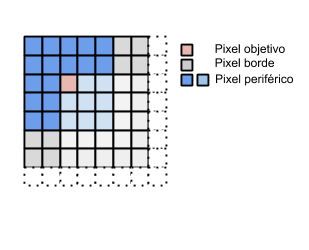
\includegraphics[scale=1]{imagenes/bordes-matriz-super.png} 

Los coeficientes de la matriz, siendo valores comprendidos entre 0 y 1, requeririan la utilizacion de valores de punto flotante. Al ser las operaciones con los mismos mas caras en tiempo, se pasan los numeros a valores enteros, multiplicando los flotantes por 100. La presicion del resultado se conserva porque los coeficientes son de presicion centesimal.
\\
Para no aumentar el brillo de la imagen se divide por la suma de todos los coeficientes de la matriz (6) .A esto se le agrega la division por 100 para generar los valores correctos.


\subsubsection{Descripcion del algoritmo}
\par
\bigskip
Para la descripcion del algoritmo contamos con el pseudocodigo acotado de la solucion implementada, el cual servira de guia para la interpretacion de las tareas realizadas. La logica del mismo 
fue pensada para tamaños de imagenes a partir de 5 x 5 pixeles en el caso de C y  5 x 7 en el caso de assembler. Para explicar el algoritmo se describira en primera instancia la idea y consideraciones generales que comparten ambas versiones; para luego profundizar en cada una, detallando en la seccion de assembler, los cambios realizados para la adaptacion a las instrucciones SIMD.
\par
\bigskip
\lstinputlisting[language=C,tabsize=4, numbers=left, numberstyle=\tiny\color{black},mathescape=true, backgroundcolor=\color{gray}, rulecolor=\color{black}, keywordstyle=\color{blue}, commentstyle=\color{dkgreen},stringstyle=\color{mauve}, numbersep=5pt, basicstyle=\scriptsize]{fuentes/pseudominiature_filter_c.c}

\begin{enumerate}
\item \textbf{La matriz de coeficientes} \\
La matriz, como fue dicho en la introduccion, al ser simetrica posee solo 6 valores distintos entre si: 0.01, 0.5, 0.18, 0.32, 0.64 y 1. Estos valores son guardados en forma entera multiplicandolos por 100, sin perder presicion.\\

\item \textbf{Recorrido de la imagen} \\
En una primera implementacion se recorria la matriz de pixeles en forma lineal (tomando la matriz como una lista). No obstante se vio que la lectura y desarrollo del codigo se complicaba a la hora de calcular limites y casos bordes, al contrario de un recorrido por filas y columnas.\\

\item \textbf{Posicion del pixel en la matriz} \\
Al hacerse un recorrido por filas y columnas es necesario un calculo adicional para traducir la posicion: por lo que la posicion se calcula haciendo columna * tamPixel + fila * width * tamPixel, siendo tamPixel = 3 (imagen en RGB).\\

\item \textbf{Limites de bandas e iteraciones} \\
Los limites de las bandas por iteracion fueron dados por consigna mediante la aplicacion de una ecuacion que presenta una division. No estaba especificado lo que se debia hacer en caso de que la misma no fuese exacta (con resto). Se pudo determinar en la etapa de testeo, que en el caso de la bada superior, se debia redondear para arriba. Este cambio se realizo al notar que solo el ultimo test: test-miniature-03-08-5-city; aparecian en el primer frame procesado, en la banda superior, una diferencia en las imagenes por 2 pixeles. Al aumentar la cantidad de iteraciones del test y bajar la tolerancia en la comparacion, se pudo determinar que en las bandas de las iteraciones de division no exacta, se perdia una linea de pixeles. El cambio permitio pasar 29 frames del test final.
 Otros pxeles fueron marcados como diferentes en la esquina inferior del frame 30. Se intento la aplicacion de la misma solucion que para el caso anterior pero sin exito. Al ser los ultimos pixeles filtrados de la imagen (5 pixeles diferentes), y ser objetivo de varias iteraciones, se supuso  algun tipo de error numerico entre nuestra version y la version que produjo las imagenes del test. Se descarto la posibilidad de perdida de presicion ya que en las operaciones para adaptar los coeficientes a valores enteros, no se recorto ninguna cifra y en las operaciones se cuido de no producir redondeos de mas.
\\

\item \textbf{Bordes de la imagen} \\
El algoritmo solo se puede aplicara a los pixeles cuya posicion diste en 2 de los bordes de la imagen. No obstante, en la etapa de testeo se determino que, para pasar exitosamente los tests, se debia considerar los pixeles a partir de la fila 4\\

\item \textbf{Intercambio} \\
Para aumentar el efecto del blureado se pasa la imagen blureada a la proxima iteracion como imagen fuente.\\

\end{enumerate}

Hasta este punto el algoritmo implementado en C y en Assembler son iguales. La diferencia entre ellos radica en la implementacion de \textbf{aplicarFiltro} y \textbf{copiarIgual}\\

\subsubsection{Implementacion en C}

Tanto en la aplicacion del filtro como en la copia de los pixeles se hace un procesamiento por pixel, es decir, se lee un pixel se copia un pixel.Como para cada pixel a filtrar son necesarios 2 filas de pixeles circundantes, la imagen mas chica a evaluar debera tener por lo menos una dimension de 5 x 5 pixeles.

\lstinputlisting[language=C,tabsize=4, numbers=left, numberstyle=\tiny\color{black},mathescape=true, backgroundcolor=\color{gray}, rulecolor=\color{black}, keywordstyle=\color{blue}, commentstyle=\color{dkgreen},stringstyle=\color{mauve}, numbersep=5pt, basicstyle=\scriptsize]{fuentes/pseudo-filtro-mini.c}

\par
\bigskip
El filtro obtiene un cuadrado de pixeles de 5 x 5 tomando como centro el pixel a blurear y a cada pixel, dependiendo su posicion se lo multiplica con un coeficiente de la matriz. El resultado se guarda en una variable temporal por cada color del pixel. Al finalizar de multiplicar a todos los pixeles del cuadrado, normalizamos por 600 (6 del brillo y 100 por la conversion a enteros).

Este procedimiento se realiza 25 veces, que es la cantidad de pixeles dentro del cuadrado. Finalmente se escribe el pixel objetivo en el archivo de destino.

\subsubsection{Implementacion en assembler utilizando set de instrucciones SIMD}

Al disponer de instrucciones que nos permiten paralelizar calculos, se busco la forma de juntar el procesamiento de las partes del algoritmo en donde se analizaba de a un dato. Este aspecto es fundamental, ya que nos permite disminuir los accesos a memoria, principal cuello de botella de C. La idea implementada con SIMD se dividio en 2 aspectos del algoritmo: la copia de pixeles iguales, como los bordes y el frame central, y el filtrado de aquellos pixeles de las bandas superior e inferior. Incluido en la optimizacion de accesos a memoria, se busco, aparte del copiado de mas de un pixel a la vez, optimizar los calculos con la matriz, dado que representa el grueso de peticiones a memoria de nuestra solucion.

Al estar trabajando con mas de un dato, surgieron casos bordes y detalles que en C, no habia. En los siguientes puntos se muestran los distintos aspectos que fueron adaptados para el uso de las SIMD.

\textbf{Copia de pixeles:}

Para la copia de pixeles iguales se aprovecho el hecho de que los pixeles levantados son consecutivos, por lo que se pudo copiar de a 5 pixeles enteros por acceso a memoria. Esto se debe al uso de los registros de 16 bytes, (descartandose el ultimo byte).

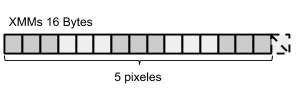
\includegraphics[scale=0.7]{imagenes/xmm-pixeles.png} 
\\
\textbf{Caso borde:}
\\
Bajo este modo de copia surge un caso borde al final del archivo de imagen. Como se esta levantando de a 16 bytes, el archivo puede no ser divisible por dicho numero (en la mayoria de los casos), con lo cual se debe detectar la proximidad al final del archivo y correr el puntero de la memoria a levantar 16 bytes antes del borde.

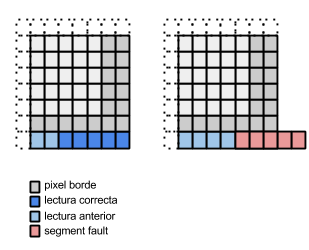
\includegraphics[scale=0.7]{imagenes/caso-borde-5.png} 

\textbf{Filtro:}
\\
Para la implementacion del filtro en Assembler se realizaron 2 etapas: Paralelismo en cuanto a calculo con la matriz de coeficentes y paralelismo en cuanto a pixeles copiados.
\par
\bigskip
La primera etapa busco reducir el numero de accesos de memoria para el calculo del producto de los coeficientes de la matriz con los pixeles circundantes al objetivo. Se aprovecho el hecho de que la longitud de las filas de la matriz y la cantidad de pixeles levantados por XMMs coincidian, con lo cual se procedio a calcular el resultado parcial de los productos y sumas de cada fila. Luego se normalizaba con 600 y se pasaba el valor del pixel a memoria:

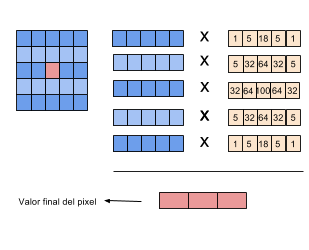
\includegraphics[scale=0.7]{imagenes/version1-miniature.png} 

De esta forma estariamos levantando de memoria 5 veces por cada pixel evaluado, con lo que reduce los 25 accesos por pixel de la version en C.

La segunda tapa fue la de lograr incorporar mayor cantidad de pixeles al resultado. Por razones de cantidad de registros se logro procesar un maximo de 3 pixeles a la vez. Esto se alcanza mediante el solapamiento de cuadrados de 5 x 5 de los 3 pixeles:

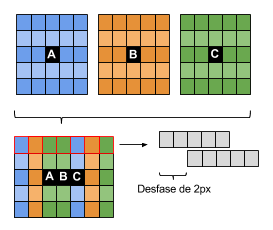
\includegraphics[scale=0.7]{imagenes/solapamiento-cuadros.png}  Filtro miniature: Imagen de solapamiento de datos y aprovecahmiento de xmms

De esta forma se estarian efectuando 10 accesos a memoria por cada 3 pixeles evaluados. En cuanto el archivo de entrada debera contar ahora con 2 columnas mas, aumentando a 5 x 7 la menor imagen filtrable por el algoritmo
\\
\textbf{Caso borde:}
\\
Al igual que en la copia de pixeles, el filtrado posee un caso borde en la ultima fila que puede ser filtrada: la antepenultima. Como para el procesamiento del pixel son necesarias las dos filas inferiores al pixel y las dos columnas del borde, si no se detecta a tiempo se produce un error de acceso a segmento. Esto se evita añadiendo logica de borde la cual, de estar analizando alguna de los ultimos 3 pixeles filtrables, se tome el puntero de memoria a levantar de forma que en el calculo de levantado de las filas para los coeficientes, no nos genere un error de segmento:\\

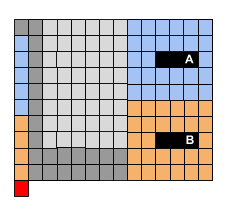
\includegraphics[scale=0.7]{imagenes/caso-borde-filtrar.png} 

En la imagen anterior, se pueden ver dos situaciones. El cuadro de pixeles donde se encuentra el pixel A, llego a un borde y lee datos basura del otro borde de la matriz. Sin embargo esto no presenta ningun problema, ya que, los pixeles leidos existen y el dato erroneo del pixel A que se guarda en la nueva imagen, sera pisado cuando el algoritmo detecte en una iteracion siguiente de que pertenece al borde (explicado en seccion siguiente), por lo que copiara nuevamente a la posicion de destino el valor correcto.

En el caso B se puede ver que se ha llegado al final de la imagen, por lo que, al contrario del caso A, si leo un pixel del borde, no va a ver una fila inferior para leer, con lo que nos iriamos del segmento. Para contrarrestar esto, la logica de borde analiza que de estar en la antepenultima fila filtrando y si estamos en el antepenultimo pixel que se debe filtrar, levante y procese los 3 pixeles, se saltee directamente los 2 proximos pixeles (ultimo y anteultimo, porque de no saltearlos en la proxima iteracion volveriamos al caso borde creanso un loop infinito) y adelante el cursor de columna directamente a los pixeles del borde.


\textbf{Solapamiento entre filtrado y copiado:}
\\
Al estar analizando de mas de un pixel a la vez, se da la situacion en que: por ejemplo, al levantar 5 pixeles para copiar y dejar igual, estemos levantando uno o varios que deben ser filtrados, con lo cual de pasar a analizar los proximos pixeles, estariamos produciendo una imagen con error. 

Para evitar esto estamos obligados a analizar indice de pixel a indice, determinando en cada caso cuando debemos filtrar y cuando no. Para seguir con la idea del procesamiento de 3 pixeles (o 5 en el caso de copia sin modificacion) establecemos un contador el cual no indica cuantos pixeles fueron analizados previamente. Si al analizar un pixel el contador no esta en cero, entonces podemos evitar la lectura de memoria de ese pixel. Al estar escasos de registros de proposito general, se utilizo un solo registro para llevar el contador de ambos: el mismo toma valores de 0 a 5 en caso del levantamiento por copia, y de 6 a 8 para los filtrables: 

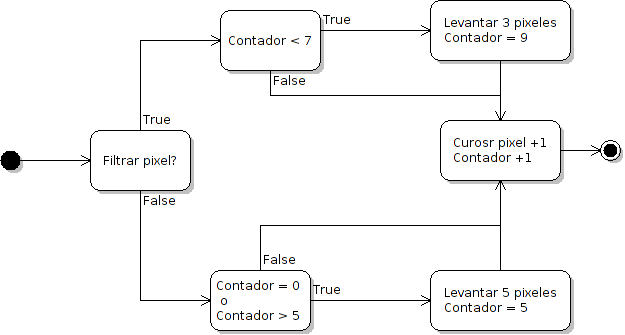
\includegraphics[scale=0.5]{imagenes/uml-mini.png}



\subsubsection{Detalle de procesamiento de filtrado de a 3 pixeles}

Suponiendo a los pixeles A, B, C, pixeles a ser filtrados, vamos a detallar el calculo de los colores. Para el procesamiento se va a necesitar un rectangulo de pixeles que contendra toda la informacion que necesitamos evaluar para el resultado final. Cada fila de este rectangulo se puede obtener mediante 2 accesos de memoria, como puede verse en la imagen anterior de solapamiento de datos.\\

Los datos obtenidos en estos 2 registros son utiles para el calculo de cada uno de los 3 pixeles, siendo utiles para mas de uno a la vez, con lo cual, se los debe multiplicar por mas de un coeficiente distinto.

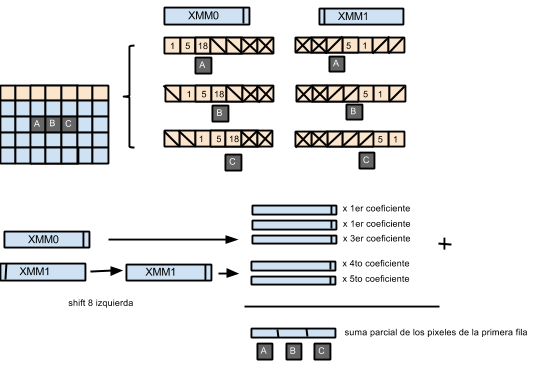
\includegraphics[scale=0.8]{imagenes/mini-matriz-descomposicion.png}

Como cada resultado de cada coeficiente le es util de forma ordenada a cada pixel objetivo de forma vertical, se puede aprovechar su uso para un procesamiento en paralelo. Como puede verse en la imagen anterior, en el caso del coeficiente 1 en el XMM0, multiplica el primer, segundo y tercer pixel. Usando esto, podemos multiplicar directamente a todos los pixeles de la fila (osea a cada color) por el coeficiente y sumarselo a las sumas parciales de cada uno de los 3 pixeles objetivo (ya que estamos usando solo 3 pixeles en cada levantada del XMM0 y XMM1).

En el caso del primer coeficiente, los pixeles quedan justo alineados para sumar al resultado parcial. Esto no ocurre para los demas, estando para el segundo coeficiente desfasados en un pixel y para el tercero en 2. Para el 4to y quinto los pixeles se recuperan en un segundo XMM, el cual tiene un corrimiento de 1 pixel y 2/3 para levantar de memoria. Se hace de esta forma, con 1/3 (8 bits) de pixel anterior leido al principio para que todo lo levantado por los XMM sean datos validos y a usar en los calculos del filtro. Este corrimiento de 1/3 se  compensa corriendo los datos del XMM 8 bits, ya que es un dato que ya se uso para los coeficientes anteriores, y no es necesario para los calculos del 4to y 5to, puede ser ignorado.

Al finalizar la multiplicacion por cada coeficiente (cuyo resultado esta en las primeras 3 posiciones del XMM) solo falta la suma con las sumas parciales guardadas anteriormente y luego pasar a la segunda fila. Para cada fila la logica del procedimiento es equivalente. En lo unico que varia es el los coeficientes de cada posicion y en el corrimiento por fila para levantar los datos de la matriz.

Al finalizar el procesamiento de los pixeles debemos dividir por el coeficiente normalizador (6) y el ajuste por considerar integer a los coeficientes de la matriz (100) y finalizar ordenando los pixeles obtenidos para escribirlos en memoria.\\


Para hacer estas multiplicaciones, sumas y divisiones en paralelo se tuvo que tener en cuenta la perdida de presicion de datos. Dado que cada color esta representado en 8 bits, al multiplicarlo por un valor entero se corre el riesgo de un overflow. El maximo numero posible con los coeficientes de la matriz estaria representado por el color 255 y el coeficiente 1 (osea 100) con lo cual tendrriamos al 25500 como supremo y maximo del conjunto, que entra en un tamaño de word.\\



Para la suma de cada colr esta sumando el valor de 25 words con un valor maximo de 25500 con lo cual se tendria como nueva cota a 637500, el cual entra en un tamaño de doubleword. Por esta razon, la suma total de cada pixel estaria representada por 3 doublewords, con lo cual el resultado de los 3 pixeles entra en 3 XMM, teniendo en el ultimo de ellos solo la primera doubleword con datos de color.\\

La operacion de desempaquetamiento se hace en otro orden, respetando la misma idea: primero se descomprimenl los 8 bits de cada color a word. Ahora se usa la operacion PMULLW y PMULLHW, las cuales hacen una multiplicacion de a word y devuelven un doubleword.. que seria exactamente lo que se necesita en este caso, ahorrandosse un paso de desempaquetamiento:\\


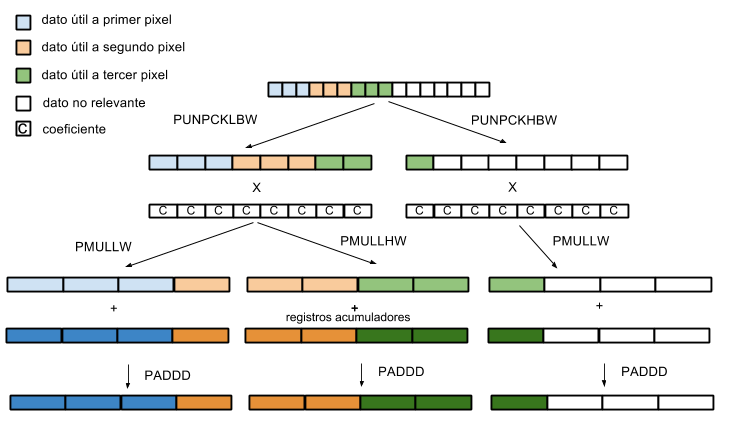
\includegraphics[scale=0.5]{imagenes/operaciones-xmms-fila.png}




El siguiente paso es convertir estos 3 registros de double words en 1 de 16 bytes en donde los colores esten en orden, al igual que los pixeles para asi poder pasarlos de una a memoria.

Para esto primero vamos a normalizar el resultado por 600. Como se busca hacerlo en paralelo, genero un registro con 600 repetido en cada double word y divido de forma paralela. Para ello necesito pasar antes a punto flotante para poder usar las funciones SIMD, y luego retornar los valores a enteros. Con la operacion DIVPS pasamos a dividir los floats por floats empaquetados, luego con la operacion CVTDQ2PS recuperamos el resultado de las divisiones con redondeo por truncamiento a doubleword integers.


Teniendo ya los resultados finales, lo que falta es la reconversion a 8 bit de cada color.
Para los 2 primeros registros de resultados podemos empaquetar ambos registros a word con una sola instruccion (PACKSSDW) y de word a byte con otra (PACKUSWB):\\

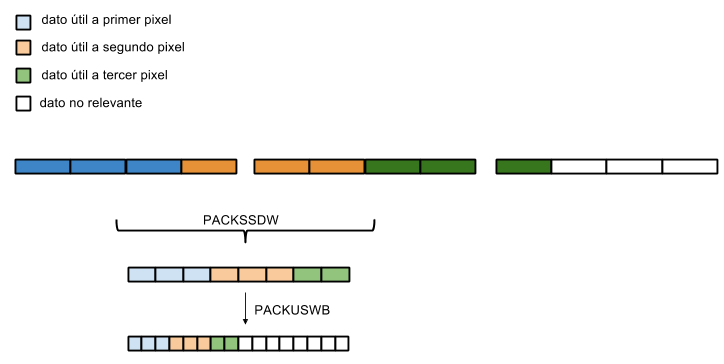
\includegraphics[scale=0.5]{imagenes/empaquetamiento.png}

Como se puede ver en la imagen anterior, aun queda un color del ultimo pixel en el ultimo registro, con lo cual debemos insertarlo en el registro de retorno para poder guardarlo en memoria.

Para lograr esto vamos a hacer uso de una mascara que nos aislara el color en la posicion en la cual tengamos que insertarlo en el registro destino. El valor a aislar, aunque sea double word, vale notar que su valor no supera a 255, ya que posee el valor de un color valido, por lo que el numeo en integer ocupa el tamaño de 8 bits. Gracias a esto se lo puede considerar tambien como un word integer y usar la instruccion PINSRW para insertar en el lugar indicado del registro el valor. Al registro destino se le setearan los bits en 0 en el lugar donde tengamos que insertar el valor resagado y mediante una suma logica vamos a pegar el color en el lugar correspondiente. Al entrar en un byte el valor pegado, los ceros de la parte alta del word no cambian los valores anteriormente empaquetados.\\

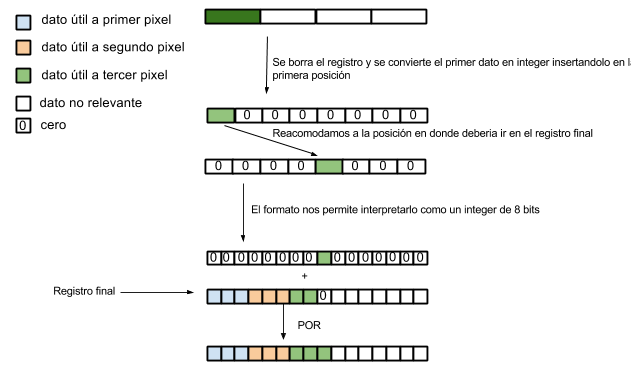
\includegraphics[scale=0.5]{imagenes/reacomodamiento.png}

\subsubsection{C vs Assembler con SIMD}

Las diferencias mas fuertes en la estructura del algoritmo en las implementaciones pueden reducirse a 2, y dejar las demas como consecuencias de estas: La cantidad de datos procesados y accesos a memoria. Como se explico anteriormente, la resolucion en C debe hacer 25 accesos a memoria por pixel filtrado y un acceso por pixel copiado (el que lo pasamos directo). Por otro lado, el algoritmo de assembler logra reducir los accesos a 10 por cada 3 pixeles evaluados, gracias al solapamiento de los cuadros de pixeles y la capacidad de los registros XMM de obtener de a tandas de 5 pixeles. Por esto tambien se pudo reducir los accesos para dejar pixeles iguales, copiando de a 5 pixeles por vez, la velocidad del algoritmo aumenta drasticamente por la manipulacion en paralelo de estos datos que no necesitan procesamiento alguno. Los resultados pueden ser vistos en los siguientes graficos que comparan la cantidad de ciclos consumidos por el CPU para 2 archivos distintos corridos sobre C y sobre assembler:


\subsubsection{Tiempos de ejecucion de diferentes experimentos}

\par
\bigskip
\textbf{Caracterizacion del experimento: }
\begin{itemize}
    \item \textbf{Iteraciones: } 5
    \item \textbf{Comando C City: }  ./tp2 -t 5 miniature -i c city.avi 0.3 0.8 3
    \item \textbf{Comando ASM City: }  ./tp2 -t 5 miniature -i asm city.avi 0.3 0.8 3
    \item \textbf{Comando C Ink}./tp2 -t 5 miniature -i c ink.avi 0.3 0.8 3
    \item \textbf{Comando Asm Ink}./tp2 -t 5 miniature -i asm ink.avi 0.3 0.8 3
\end{itemize}
\par

\textbf{Resultados:}\\
\begin{center}
    \begin{tabular}{|l|l|l|l|l|}
        \hline
        Medición  & C ink.avi  & ASM ink.avi & C city.avi  & ASM city.avi \\
        \hline
        Ciclos por llamada	&	459987456	& 76210288 & 459888288 & 76193352 \\
        \hline
    \end{tabular}
\end{center}
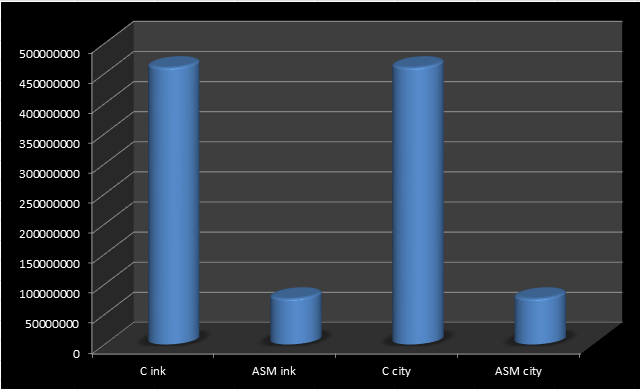
\includegraphics[scale=1]{imagenes/miniature-grafico.png} 

\subsubsection{Comentarios sobre los resultados obtenidos del experimento}

Las diferencias impactan notablemente sobre los tiempos de ejecucion del algoritmo aumentando notoriamente la velocidad de procesamiento de los videos objetivos en un \%600. De esta forma se puede concluir que a la hora del procesamiento de archivos de medios, las instrucciones SIMD logran un mejor aprovechamiento del poder de computo del CPU al permitirnos manipular mayor cantidad de datos y de forma paralela sobre memoria disminuyendo los accesos a ella.

\newpage